\chapter{Základné pojmy}

\section{Futbal}
Futbal je šport, pri ktorom na hracej ploche, futbalovom ihrisku (na obrázku \ref{pitch}), proti sebe nastúpia dva jedenásťčlenné tímy s cieľom skórovať čo najviac gólov a inkasovať čo najmenej.
Na ihrisku je vždy najviac jedna lopta, hráči ju ovládajú prevažne nohami. 
Gól nastáva, keď jeden s tímov pošle loptu celým objemom za bránkovú čiaru do priestoru medzi bránkové tyče, teda do súperovej bránky, vrámci pravidiel. 
Víťazom sa stáva tím, ktorý strelí viac gólov ako súper. 
Ak je počet vstrelených gólov pre obe zúčastnené strany rovnaký, nastáva remíza 
\citep{hry1}.
\noindent
\begin{figure}[h!]
\centering
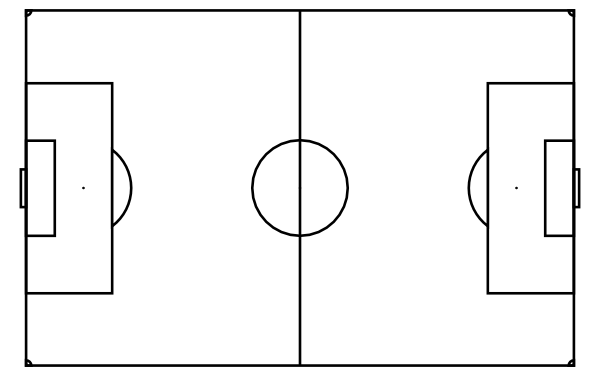
\includegraphics[scale=0.3]{../img/pitch.png}
\caption{Vzhľad futbalového ihriska, pre medzinárodné zápasy musí mať dlhšia strana 115 -- 120\,m, kratšia 64 -- 95\,m} 
\label{pitch}
\end{figure}

\subsection{Futbalové ligy}
Väčšina futbalových líg na svete (vrátane tých, s ktorými sa pracuje v tejto práci) funguje aspoň z časti sezóny na systéme, ktorý môžeme nazvať \textit{každý s každým}.
To znamená, že každý tím odohrá zápas proti každému tímu v lige.
Každá sezóna týchto líg sa najprv delí na kolá a až potom na zápasy.
V každom kole odohrá jeden zápas každý tím (s výnimkou jedného tímu, ak liga obsahuje nepárny počet tímov, ten má v danom kole voľno).
Za výhru v každom zápase sú 3 body, za remízu 1 bod a za prehru nedostane tím žiaden bod.
Sledované ligy fungujú na barážovom systéme, teda najnižšie umiestnené tímy zostupujú do nižšej ligy v hierarchii líg v danej krajine a najvyššie umiestnené tímy postupujú do vyššej ligy v hierarchii.

\section{Tenis}
Tenis je šport tímov súperiacich proti sebe, skladajúcich sa z jedného alebo dvoch ľudí, hrajúcich proti sebe na tenisovom kurte.
Zápasy sa delia na dvojhry, teda zápasy dvoch jednočlenných tímov, a štvorhry, zápasy dvoch dvojčlenných tímov.
Hlavným cieľom tenisu je použiť tenisovú raketu na zahratie loptičky na súperovu stranu kurtu (obrázok \ref{court}) jedným úderom tak, aby mala súperiaca strana, čo najväčší problém ho vrátiť naspäť \citep{tenis:kor}. 
Ak sa to jednému z tímov nepodarí v súlade s pravidlami, súper získa bod.
Tím, ktorý získa 4 body, získa hru. Ak obe tímy získajú po 3 body skôr, ako jeden z nich získa 4, hru získa tím, ktorý získa o 2 body viac ako súper.
Tím, ktorý skôr získa 6 hier, získa sadu. Ak nastane stav 5:5, hru získa tím, ktorý získa 7 hier.
Zápas sa hrá na dve alebo tri víťazné sady, toto číslo je vždy určené vopred.
V tejto práci nás budú hlavne zaujímať dvojhry, teda zápasy jeden proti jednému.
\citep{hry2}.

\noindent
\begin{figure} [h!]
\centering

\includegraphics[scale=0.7]{../img/court.png}
\caption{Vzhľad tenisového kurtu, kurt je dlhý 23,77\,m, široký 10,97\,m, dodatočný prázdny priestor okolo kurtu je vyhradený, aby hráči mali možnosť dosiahnuť na loptičky, ktoré sú v hre, ale nachádzajú sa mimo kurtu. Sieť je vysoká 1.07\,m na krajoch kurtu, 0,91\,m v strede.}
\label{court}
\end{figure}

\subsection{Turnaje ATP Tour}
ATP Tour je tenisový okruh najvyššej celosvetovej úrovne organizovaný asociáciou ATP (Association of Tennis Professionals).
Profesionálni hráči sa schádzajú na turnajoch po celom svete.
Tieto turnaje sa hrajú vyraďovacím systémom, teda hráč ktorý vyhrá v zápase postúpi do ďalšieho kola turnaja až do finále.
Pár najvyšších hráčov postúpi priamo do vyraďovacej časti turnaja, ak sa doň prihlásia, zvyšní hráči ešte musia prejsť kvalifikáciou predtým, ako budú môcť hrať priamo na turnaji.
Turnaje spadajúce pod ATP Tour sú turnaje typu ATP Masters 1000, ATP 500 a ATP 250. Tieto turnaje sú nazvané podľa počtu bodov, ktoré si hráč pripíše za výhru.
Turnaje Grand Slam spadajú pod ITF (International Tennis Federation), víťaz ale za víťazstvo na týchto turnajoch dostane 2000 bodov.
ATP publikuje rebríček profesionálnych hráčov týždenne, hráči sú zoradení zostupne podľa počtu získaných bodov v poslednom roku.


\section{Porovnanie futbalu a tenisu}
Z predchádzajúcich kapitol je zrejmé, že futbal a tenis majú veľa spoločných a veľa rozdielnych vlastností. 
Futbal je kontaktný šport, teda protihráči sú často vo fyzickom kontakte medzi sebou, zatiaľ čo pri tenise sú protihráči vždy na opačných stranách tenisového kurtu. 
Rozdielny je aj počet hráčov v jednom tíme, vo futbale je maximálny počet hráčov hrajúcich v jednom momente za jeden tím 11, v tenise to je buď jeden alebo dvaja.
Spoločný je napríklad fakt, že sa jedná o loptový šport. 
Na druhej strane, vo futbale je povolené loptu zasiahnuť ktoroukoľvek časťou tela okrem rúk (s výnimkou brankára), v tenise je zakázané dotknúť sa tenisovej loptičky akoukoľvek časťou tela, loptičku je povolené zahrať len tenisovou raketou.
Ďalším rozdielom je hrací čas. Vo futbale má každý zápas fixnú dĺžku (2 polčasy po 45 minút s maximálne 15 minútovou prestávkou medzi nimi), rozhodca na konci každého polčasu nadstaví čas, po ktorý sa nehralo kvôli rôznym prerušeniam v hre 
\citep{hry1}.
V tenise môže zápas vďaka pravidlám trvať od desiatok minút do niekoľko hodín \citep{tenis:kor}.


\section{Kurzy stávkových na kancelárií}
Kurzové stávky sú stávky na akýkoľvek jav, na ktorý vypíše daná stávková kancelária kurz. 
Kurzy stanovuje bookmaker podľa toho, aká je pravdepodobnosť, že daný jav nastane, kde platí, že čím nižší kurz, tým je vyššia pravdepodobnosť nastania daného javu. 
Väčšinou sa tieto javy týkajú nejakej športovej udalosti, napríklad futbalových zápasov alebo automobilových pretekov. 
Stávkové kancelárie ale vypisujú kurzy aj na nešportové udalosti, kde medzi tie známejšie patria prezidentské voľby \citep{bet:pres} alebo ohlásenie mena novorodeného dieťaťa v kráľovskej rodine, kde zvyknú byť vypísané kurzy napríklad na pohlavie, meno novorodenca alebo presný dátum narodenia \citep{bet:prince}.

Na javy, na ktoré sú vypísané kurzy, môže potom zákazník staviť istú sumu peňazí, vklad, obvykle tak, že vloží tento vklad do stávkovej kancelárie. 
Ak daný jav nastane, zákazník dostane od tejto stávkovej kancelárie výhru, ktorá predstavuje výsledok vynásobenia daného kurzu vkladom.
Ak daný jav nenastane, vklad prepadá v prospech stávkovej kancelárie.
Pre príklad si vezmime tipovanie výsledku futbalového zápasu Slovensko - Česká republika, ktorý sa odohral dňa 13.10.2018. 
Podľa internetového portálu OddsPortal.com bol priemerný vypísaný kurz na tip domáci (v tomto prípade Slovensko) 2,06, na tip hostia (Česká republika) 3,86 a na tip remíza 3,35.
Zápas skončil výhrou hostí, čo znamená, že ak by sme boli stavili 100\,\rm korún na tento výsledok, tak by sme si boli odniesli zo stávkovej kancelárie 386\,\rm korún  (3,86 * 100 = 386), čo predstavuje zárobok 286\,\rm korún, pretože 100\,\rm korún predstavuje vklad.
Ak by sme boli stavili 100\,\rm korún na výhru domácich alebo na remízu, tak by sme boli prehrali celý vklad.

Stávkovanie je hazardná hra, obľúbená práve preto, že každý hráč môže vyhrať a vie aj ovplyvniť svoju pravdepodobnosť úspechu tým, že danú udalosť pozná \citep{odds}.

\begin{figure}
\centering
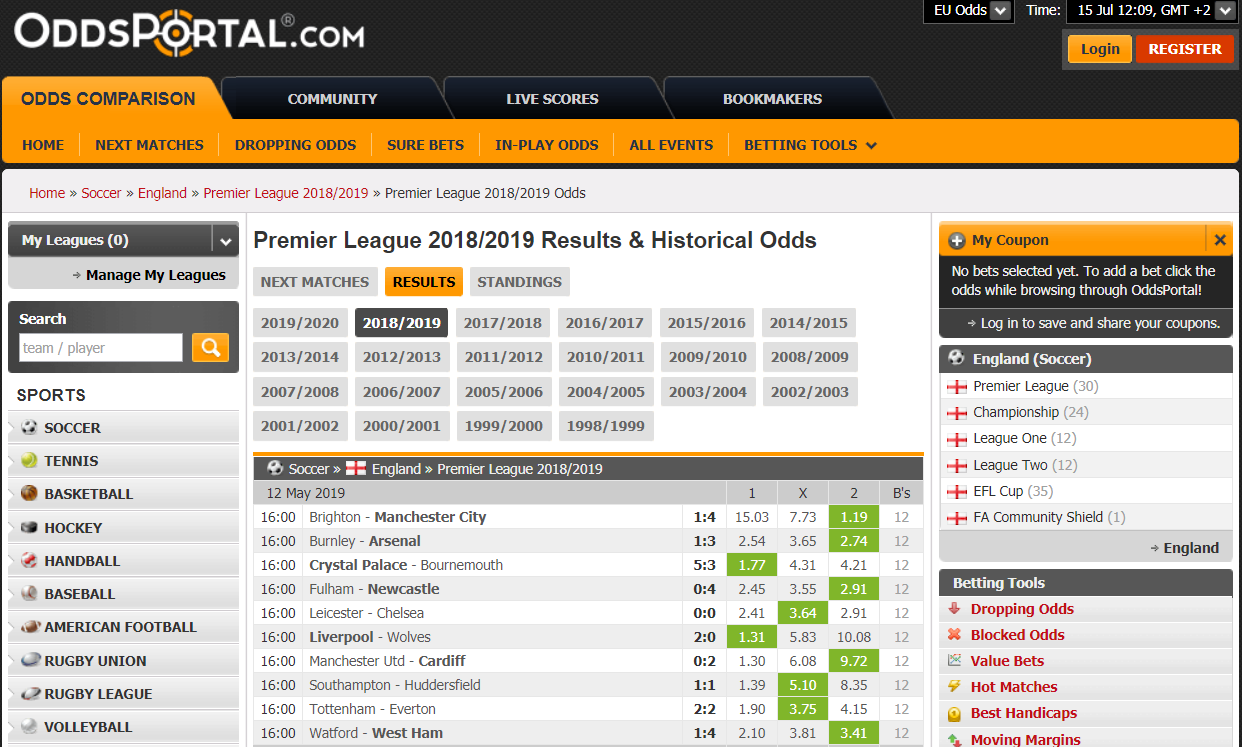
\includegraphics[width=\textwidth]{../img/odds.png}
\caption{Takto vyzerá stránka OddsPortal.com, z ktorej som získaval dáta pre potreby tejto práce. Znázornené je posledné kolo predikovanej časti anglickej \textit{Premier League}.} 
\label{odds}
\end{figure}